%%%%%%%%%%%%%%%%%%%%%%%%%%%%%%%%%%%%%%%%%%%%%%%%%%%%%%%%%%%%%%%
%%% HEADER %%%%%%%%%%%%%%%%%%%%%%%%%%%%%%%%%%%%%%%%%%%%%%%%%%%%
%%%%%%%%%%%%%%%%%%%%%%%%%%%%%%%%%%%%%%%%%%%%%%%%%%%%%%%%%%%%%%%

\documentclass{layout/si-msc-proposal}
\usepackage{float}
\usepackage{todonotes}
\usepackage{dirtytalk}
\usepackage{subcaption}
\usepackage{listings}
\usepackage{tikz}
\usepackage{color}
\usepackage{pgfgantt}
\usepackage{hyperref}

\graphicspath{ {./images/} }

\newcommand\YAMLcolonstyle{\color{red}\mdseries}
\newcommand\YAMLkeystyle{\color{black}\bfseries}
\newcommand\YAMLvaluestyle{\color{blue}\mdseries}

\makeatletter

\newcommand\language@yaml{yaml}

\expandafter\expandafter\expandafter\lstdefinelanguage
\expandafter{\language@yaml}
{
    keywords={true,false,null,y,n},
    keywordstyle=\color{darkgray}\bfseries,
    basicstyle=\YAMLkeystyle,
    sensitive=false,
    comment=[l]{\#},
    morecomment=[s]{/*}{*/},
    commentstyle=\color{purple}\ttfamily,
    stringstyle=\YAMLvaluestyle\ttfamily,
    moredelim=[l][\color{orange}]{\&},
    moredelim=[l][\color{magenta}]{*},
    moredelim=**[il][\YAMLcolonstyle{:}\YAMLvaluestyle]{:},
    morestring=[b]',
    morestring=[b]",
    literate =    {---}{{\ProcessThreeDashes}}3
        {>}{{\textcolor{red}\textgreater}}1
        {|}{{\textcolor{red}\textbar}}1
        {\ -\ }{{\mdseries\ -\ }}3,
}

\setlength\parindent{0pt}

\author{Edoardo Riggio}

\title{API Scout: An Information Retrieval System for OpenAPI Specifications}

\abstract{

    The primary objective of this thesis is to create an information retrieval system enabling users to explore a compre hensive collection of OpenAPI specifications. The system will use historical versioned data - scraped from existing github repositories - as well as user-uploaded data. \\

    This platform serves a dual purpose, catering to both academics and developers. In the case of academics, this platf orm can serve as a repository from which to conduct research, facilitating more in-depth studies on API specificatio ns and their evolution. On the other hand, developers can look up several different examples that could help them get started with their own OpenAPI documentation. \\

    The main contributions of this thesis include two crucial aspects: data engineering and software engineering. In the first case, the thesis will delve in the process of refining raw data and finding ways to classify the API specifications. In the second case, the thesis will define the architectural design and the development of the service itself.
}

\begin{document}

    \maketitle

%%%%%%%%%%%%%%%%%%%%%%%%%%%%%%%%%%%%%%%%%%%%%%%%%%%%%%%%%%%%%%%
%%% MAIN BODY %%%%%%%%%%%%%%%%%%%%%%%%%%%%%%%%%%%%%%%%%%%%%%%%%
%%%%%%%%%%%%%%%%%%%%%%%%%%%%%%%%%%%%%%%%%%%%%%%%%%%%%%%%%%%%%%%

    \tableofcontents
    \listoffigures
    \listoftables
    \newpage

%%%%%%%%%%%%%%%%%%%%%%%%%%%%%%%%%%%%%%%%%%%%%%%%%%%%%%%%%%%%%%%
%%%%%%%%%%%%%%%%%%%%%%%%%%%%%%%%%%%%%%%%%%%%%%%%%%%%%%%%%%%%%%%

    \section{Introduction}\label{sec:introduction}
    In the ever-evolving landscape of software engineering, APIs play a pivotal role in facilitating the communication and interoperability between software services.
Being software systems intrinsically complex, it is good practice to keep track of the interfaces that they expose.
Moreover, especially in the cases where these interfaces have to be used by external developers, it is paramount to have good documentation for such interfaces. \\ \\
In this thesis, we will work with a specific type of API: HTTP APIs\@.
Such APIs are exposed by Web servers and accessible though HTTP requests.
To properly document public HTTP APIs, Swagger proposed in 2011 the \("\)Swagger Specification\("\) (today known as \("\)OpenAPI Specification\("\)).
As Swagger explains on its website, \("\)[t]he OpenAPI Specification (OAS) defines a standard, language-agnostic interface to HTTP APIs which allows both humans and computers to discover and understand the capabilities of the service [\dots].\("\)~\cite{swagger_openapi_2021} \\ \\
Every service with public endpoints, should expose -- as per Swagger's specifications -- a \verb|opena-| \\ \verb|pi.json| or \verb|openapi.yaml| file.
This file can be one, or it can be the root of several other smaller files -- at the discretion of the author.
Moreover, each document that specifies the endpoints' structure must be written following a specific set of rules.
Such rules are defined and explained on Swagger's \("\)OpenAPI Specification\("\) website.


    \subsection{Motivation}\label{subsec:motivation}
    From our research, we noticed that there is a void in tools and services that can be helpful in the study of the evolution and current state of HTTP APIs.
Although platforms such as SwaggerHub\footnote{https://app.swaggerhub.com/search} and APIs.guru\footnote{https://apis.guru/} already exist, they lack features that are essential for research. \\ \\
For example, they lack a proper search system.
In the previously mentioned platforms, indexing of specifications is superficial and most of the time only the title is matched with the query.
With API Scout, we want to index API specifications based not only on their title, but based on all the tags containing natural language. \\ \\
Another feature missing in the aforementioned platforms is a proper visualization system.
By using tools to convert specifications into interactive trees, users can better understand the structure of the service's endpoints.
Moreover, we can also plot some statistics about the selected API and how it compares to all the specifications present on our platform.

    \subsection{Objective}\label{subsec:objective}
    The goal of this thesis is to build a platform that both academics and developers can use to understand and study the intricacies of real-world HTTP APIs. \\ \\
In the case of the developers, they can search and consult our historical and current collection of APIs to better understand how to structure one.
Aided by the graphical tools, a developer can also understand how the endpoints should be structured to obtain a more cohesive structure. \\ \\
On the academic side, this tool can be used to perform research on the evolution of HTTP APIs in time.
By offering historical data as well as current data, researchers can have a better understanding of how endpoints and data structures change over time as a service grows in complexity.
Researchers can also use plots and statistics pre-computed by our platform to understand how an API specification relates to the plethora of specifications present.

%%%%%%%%%%%%%%%%%%%%%%%%%%%%%%%%%%%%%%%%%%%%%%%%%%%%%%%%%%%%%%%
%%%%%%%%%%%%%%%%%%%%%%%%%%%%%%%%%%%%%%%%%%%%%%%%%%%%%%%%%%%%%%%

    \section{Proposal}\label{sec:proposal}

%%%%%%%%%%%%%%%%%%%%%%%%%%%%%%%%%%%%%%%%%%%%%%%%%%%%%%%%%%%%%%%
%%%%%%%%%%%%%%%%%%%%%%%%%%%%%%%%%%%%%%%%%%%%%%%%%%%%%%%%%%%%%%%

    \section{State of the Art}\label{sec:state-of-the-art}

    \subsection{OpenAPI Specification}\label{subsec:openapi-specification}
    An API is a set of interfaces that can be accessed by other users or developers.
To document such APIs, API specifications are used.
These specifications document the functioning and expected output of such interfaces.
% TODO - Add citation
The OpenAPI Standard~\cite{} is a specification language that offers a standardized way of writing API specifications for HTTP-based APIs.

    \subsection{Document Embedding}\label{subsec:indexing-and-searching}
    To find the most similar documents to a user-defined query, we need a way of comparing documents and defining what do we mean by similar.
First of all, we need to represent documents in a more mathematical way.
For this task, a document embedding model is employed -- we used the Universal Sentence Encoder~\cite{cer2018universal}.
This encoder will transform a document into a vector of numbers.
These vector of numbers are then stored somewhere -- ideally a database -- and assigned a name. \\ \\
When a user wants to search for a specification, we have to use the document embedding model for the query, and then retrieve the top \textit{K} documents that are the most similar to the vectorized query.
The similarity of two documents is defined by how much the two vectors (the one of the query and the one of the document) are distant from one another.
The more the two vectors are close to each other, the more they are similar.
To find out the \textit{K} nearest documents to the query, we can use the \textit{K}-Nearest Neighbors algorithm.
This algorithm will return the \textit{K} nearest documents, thus the most similar.

%%%%%%%%%%%%%%%%%%%%%%%%%%%%%%%%%%%%%%%%%%%%%%%%%%%%%%%%%%%%%%%
%%%%%%%%%%%%%%%%%%%%%%%%%%%%%%%%%%%%%%%%%%%%%%%%%%%%%%%%%%%%%%%

    \section{Preliminary Results - Feasibility Study}\label{sec:preliminary-results---feasibility-study}

    \subsection{Indexing and Searching}\label{sec:indexing-and-searching}
    With the API Scout platform being a data aggregator for OpenAPI Specifications (section~\ref{subsec:openapi-specification}), we need a way of efficiently indexing and searching through the plethora of crawled documents in our database.
When dealing with OpenAPI Specifications, we are working with JSON or YAML files (which are structured).
Moreover, these files follow the OpenAPI Specifications; thus we know that the documents will contain a very similar structure. \\ \\
Since we are dealing with a very high number of documents, it is paramount to have a fast and reliable index that can be searched through.
For this reason, we decided to use vector embeddings to represent documents in our database.
Embedding models offer a way of transforming documents into vectors of numbers, and -- in our case -- we used Google's Universal Sentence Encoder~\cite{cer2018universal} to perform the aforementioned task.
The embedding is done on only a part of the document's content, namely everything that is contained in the \verb|description|, \verb|name|, \verb|title|, and \verb|summary| labels.
We chose to do so because these labels are the only ones that contain natural language descriptions of the api in general or of api endpoints.
\begin{figure}
    \centering
    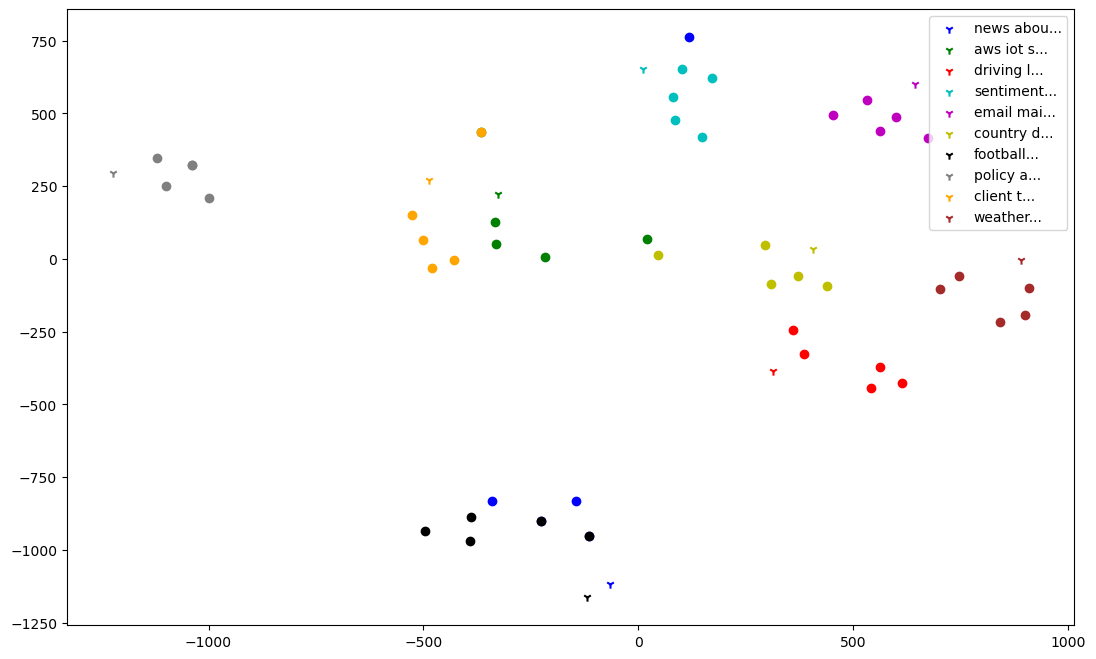
\includegraphics[width=13cm]{../out/plots/SNE}
    \caption{T-SNE Plot}
    \label{fig:tSNE-plot}
\end{figure}
After the creation of the embeddings, we saved the vectors -- as well as the name, version, and id -- of the specifications in an ElasticSearch database.
We chose ElasticSearch and the ELK (Elastic-Logstash-Kibana) stack because it is very rapid and scalable.
Moreover, ElasticSearch offers the possibility of searching documents based on the \textit{K}-NN algorithm.
This solution seems to be the most promising for the amount of data and hardware availability we have for this project.
We were considering also deep-learning models but discarded them since they are resource intensive and would be overkill for this kind of application. \\ \\
The results obtained with the embedding + K-NN solution are very promising, as we can see in Figure~\ref{fig:tSNE-plot}.
With the \("\)Y\("\) markers representing the queries, and the dots representing the most similar documents found for that query, we can see that the dots and \("\)Y\("\) markers of the same colors are fairly close to each other.
Moreover, we performed a validation step with a ground truth.
From the validation step, we concluded that the precision of the document retrieval is $p = 0.6$, while the recall is $r = 1.0$.
This validation was done on 10 different queries.
The position in which each ground truth appeared in the searches can be found below.
\begin{verbatim}
  Position in which the ground truth was found:

      "NFL v3 Ply-by-Play" was found at position #1
      "AWS IoT Secure Tunneling" was found at position #4
      "Transport Department" was found at position #4
      "Text Analytics & Sentiment Analysis API | api.text2data.com" was
        found at position #4
      "MailboxValidator Free Email Checker" was found at position #1
      "Interzoid Country Data Standardization API" was found at position #1
      "Soccer v3 Projections" was found at position #1
      "PolicyClient" was found at position #1
      "NetworkManagementClient" was found at position #3
      "Interzoid Get Weather City API" was found at position #2
\end{verbatim}
As we can see, all ground truths we found in the top 5 results -- hence $p = 1.0$.
The validation on the ground truth, though, does not paint the full picture of the capabilities this solution offers.
For example, if we try searching using the query: \("\)american sports news\("\), the top 5 documents returned by the information retrieval system will be the following.
\begin{verbatim}
  These are the top 5 results of the query "american sports news":

      1. NFL v3 Play-by-Play     v.1.0   [67%]
      2. News Plugin             v.1     [66%]
      3. Soccer v3 Projections   v.1.0   [64%]
      4. MLB v3 Projections      v.1.0   [64%]
      5. NFL v3 Scores           v.1.0   [64%]
\end{verbatim}
As we can see in the results above, the engine is able to recognize that both the \textit{NFL} and the \textit{MLB} are professional American sport leagues.
The former being the National Football League, and the latter being the Major League Baseball.
Moreover, it is also able to understand that soccer is a sport and return it. \\ \\
As can be seen both in the precision ($p = 0.6$), and the above example, there are still some noisy results that match part or none of the query, but this is acceptable.
The reason is that this is not the only means of searching.
In tandem with the natural language query, there is also a DSL that can be used to filter the documents and obtain a more accurate result.


%%%%%%%%%%%%%%%%%%%%%%%%%%%%%%%%%%%%%%%%%%%%%%%%%%%%%%%%%%%%%%%
%%%%%%%%%%%%%%%%%%%%%%%%%%%%%%%%%%%%%%%%%%%%%%%%%%%%%%%%%%%%%%%

    \section{Work Plan for the Spring semester}\label{sec:work-plan-for-the-spring-semester}
    This section describes a high level view of the work plan for the spring semester.

\begin{itemize}
    \item Iteration 1: Data Analysis Phase
    \begin{itemize}
        \item Task 1: Setup project (Pick tools/technologies to use)
        \item Task 2: Design of metrics to locate changes in evolution
        \item Task 3: Setup database of metrics
        \item Task 4: Classification of changes
        \item Task 5: Evaluate and improve system
    \end{itemize}
    \item Iteration 2: Visualization Phase
    \begin{itemize}
        \item Task 1: High level visualization of API
        \item Task 2: Drilled down visualization of API
        \item Task 3: Visualizing changes
        \item Task 4: Evaluate and improve system
    \end{itemize}
    \item Iteration 3: Report
\end{itemize}
\resizebox{\textwidth}{!}{
    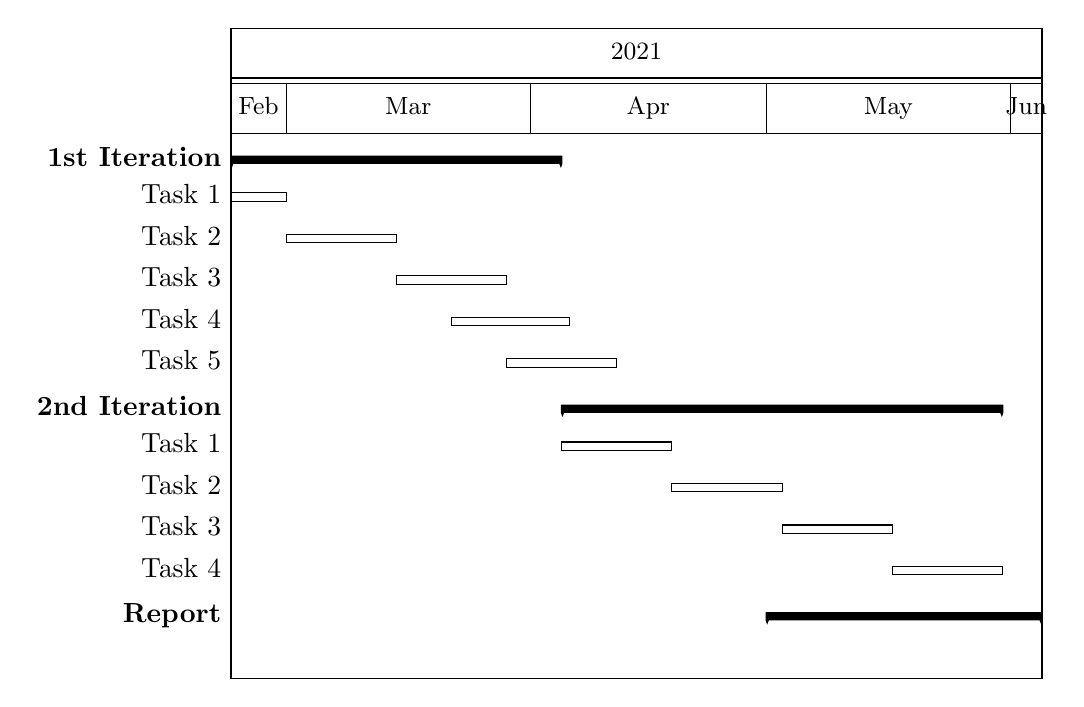
\begin{tikzpicture}
        \begin{ganttchart}[
            Mile1/.style={milestone/.append style={fill=red}},
            x unit=1mm,
            time slot format=isodate,
            y unit title=20,
            title height=.9,
            bar height=0.2,
            y unit chart=15,
        ]
        {2021-2-22}{2021-6-4}

            \gantttitlecalendar{year, month=shortname} \\

            \ganttgroup{1st Iteration}{2021-2-22}{2021-4-4} \\
            \ganttbar{Task 1}{2021-2-22}{2021-2-28}\\
            \ganttbar{Task 2}{2021-2-29}{2021-3-14}\\
            \ganttbar{Task 3}{2021-3-15}{2021-3-28}\\
            \ganttbar{Task 4}{2021-3-22}{2021-4-5}\\
            \ganttbar{Task 5}{2021-3-29}{2021-4-11}\\
            \ganttgroup{2nd Iteration}{2021-4-5}{2021-5-30} \\
            \ganttbar{Task 1}{2021-4-5}{2021-4-18}\\
            \ganttbar{Task 2}{2021-4-19}{2021-5-2}\\
            \ganttbar{Task 3}{2021-5-3}{2021-5-16}\\
            \ganttbar{Task 4}{2021-5-17}{2021-5-30}\\
            \ganttgroup{Report}{2021-5-1}{2021-6-4} \\
        \end{ganttchart}
    \end{tikzpicture}
}


%%%%%%%%%%%%%%%%%%%%%%%%%%%%%%%%%%%%%%%%%%%%%%%%%%%%%%%%%%%%%%%
%%% BIBLIOGRAPHY %%%%%%%%%%%%%%%%%%%%%%%%%%%%%%%%%%%%%%%%%%%%%%
%%%%%%%%%%%%%%%%%%%%%%%%%%%%%%%%%%%%%%%%%%%%%%%%%%%%%%%%%%%%%%%

    \newpage
    \nocite{*}
    \bibliographystyle{unsrt}
    \bibliography{bibliography/bibliography}%

\end{document}